\chapter{Further Applications}\label{chap:extension}

In this Chapter, the ordered probit model is further applied to two special periods. The first section provides and discusses the main findings for the Covid-19 period. Afterwards, the second section presents the results for the financial crisis period in 2008. Both of the discussions follow the similar structure as in the main empirical result chapter.


\section{Covid-19 Period (February-April 2020)}

The Covid-19 pandemic has brought significant disturbance to (not only) the financial and economic world. Since the stock data analyzed throughout this thesis is IBM traded on NYSE, the chosen focus is on the US stock market. \citet{coxetal2020} observe the turbulance of the S\&P 500 stock market index in the period between February to April 2020: from February 19 to March 23 the index lost 33.7\%, but rose back 29\% from March 24 to April 17. Hence, the data used in this section are taken from February to April 2020 to test the reaction of our model towards these disrupting times.


Similar to the main study, this section for Covid-19 period also has two panels: one for the full-sample market microstructure study, and the other one for the forecasting study. \tabref{tab:table-12} presents the database structure. For the forecasting panel, the first ten weeks are taken for in-sample, and the last three weeks are for out-of-sample analysis.

\begin{table}[ht]
\centering
\small
\renewcommand{\arraystretch}{1.3} % Increases row height
\setlength{\tabcolsep}{10pt} % Increases column separation
\resizebox{\textwidth}{!}{%
\begin{tabular}{|c|l|c|}
\hline
\textbf{Purpose}       & \multicolumn{1}{c|}{\textbf{Timeframe}} & \textbf{Number of transactions} \\ \hline
Panel C: Total         & February 3 - April 30, 2020           & 786,598                      \\ \hline
Panel D: In-sample     & February 3 - April 11, 2020            & 660,487 (84\% of total sample) \\ \hline
Panel D: Out-of-sample & April 12 - April 30, 2020          & 126,111 (16\% of total sample)   \\ \hline
\end{tabular}%
}
\caption{Summary of Database: IBM traded on NYSE (February-April 2020).}
\label{tab:table-12}
\end{table}


\tabref{tab:table-14} shows the frequency distribution of the Covid-19 period by each category. Noticeably, although the majority of mass still cluster around zero (category 8), there are more percentage at the extreme cases (<-6 and $\geq$6). Besides, the summary statistics of the explanatory variables (lagged price changes $Z_k$, trade direction indicator $IBS_k$, signed transformed volume \(lnV_k\cdot IBS_k\) ) could be found from \tabref{tab:table-13} to \tabref{tab:table-16} in Appendix \ref{app:tables-covid}. The proportion between price traded > Miquote and < Midquote is still roughly balance (48.32\% vs. 45.55\%), and similar picture could also be detected for trade direction (52.45\% buyer-initiated vs. 48.55\% seller initiated). The average time between trade is 1.8 seconds.





\begin{table}[H]
  \centering
  \setlength{\tabcolsep}{4pt} 
  \resizebox{\textwidth}{!}{%
    \begin{tabular}{@{} r *{14}{r} @{}}
      \toprule
      \textbf{Category}      & 1    & 2       & 3       & 4       & 5       & 6       & 7       & 8       & 9       & 10   
      & 11      & 12      & 13      & 14      \\
      
      \textbf{Price Changes}   & <–6  & [–6,–5) & [–5,–4) & [–4,–3) & [–3,–2) & [–2,–1) & [–1,0)  & [0,1)   & [1,2)   & [2,3)   & [3,4)   & [4,5)   & [5,6)   & \geq6     \\
    
      \textbf{Percentage} & 2.98\% & 0.57\% & 2.04\% & 4.14\% & 2.39\% & 9.58\% & 5.71\% & 51.28\% & 9.28\% & 2.37\% & 4.04\% & 1.96\% & 0.55\% & 3.08\%\\
      \bottomrule
    \end{tabular}%
  }
  \caption{Frequencies of Partition (February-April 2020).}
  \label{tab:table-14}
\end{table}

The ordered probit model is estimated for the Covid-19 period data, detailed estimation results are reported in \tabref{tab:table-17} in Appendix \ref{app:tables-covid}. The McFadden's $R^2$ is low with 0.0914. After estimating the model with maximum likelihood, as before, the impact of sequence-of-trade and trading volume on price change are tested. The significant $\chi^2$ at 0.1\% level from \tabref{tab:table-18} again rejects the null hypothesis that there is no difference between order of trade i.e., order flow matters.


\begin{table}[H]
    \centering
    \vspace{0.5em}
    \begin{tabular}{crrl}
        \toprule
        Df & $\chi^2$ & Pr($>$$\chi^2$) \\
        \midrule
         2 & 2835.2 & $<$ 2.2e-16 *** \\ 
         \bottomrule
        \multicolumn{3}{l}{$^{***}p < 0.001$; $^{**}p < 0.01$; $^{*}p < 0.05$}
    \end{tabular}
        \caption{Sequence of Trade: Linear Hypothesis Test (February-April 2020).}
    \label{tab:table-18}
\end{table}

In \tabref{tab:table-19}, the conditional mean for each dollar trading volume case is presented. In general, the finding is consistent with the main study that larger trade size would move the next price changes upward. Noticeably, the absolute magnitude of the changes in conditional mean for both impact in ticks and impact in percent is larger than the main study period (2023). For instant, conditioning for the increasing price sequence scenario and the base price of \$500, an increase of \$1000 trading volume in Covid-19 would increase the conditional mean by 0.33 tick, while in main study period (2023) it only increases by 0.19 tick (see \tabref{tab:table-9}). Although more tests are needed to verify whether these gaps are significant or not, one possible explanation is the decrease of market liquidity on NYSE during the Covid-19 period \citep{chung&chuwonganant2023}. 






\begin{table}[H]
\centering
\begin{tabular}{lrr}
\toprule
 & \multicolumn{1}{c}{\$Volume} & \multicolumn{1}{r}{Impact} \\
\midrule
\multicolumn{3}{l}{\textbf{Increasing price sequence (1/1/1)}} \\
\addlinespace[0.5ex]
\multicolumn{3}{l}{\emph{Price impact in ticks}} \\
E$[Z_k]$             &  500   &  $0.0802$ \\
$\Delta E[Z_k]$      & 1{,}000   &   $0.1664$ \\
$\Delta E[Z_k]$      & 1{,}500   &   $0.3337$ \\
$\Delta E[Z_k]$      & 2{,}000   &   $0.5027$ \\
$\Delta E[Z_k]$      & 2{,}500   &   $0.6742$ \\
$\Delta E[Z_k]$      & 5{,}500   &   $1.7823$ \\
\addlinespace[1ex]
\multicolumn{3}{l}{\emph{Price impact in percent}} \\
E$[Z_k]$             &  500   &  $0.0006$ \\
$\Delta E[Z_k]$      & 1{,}000   &   $0.0013$ \\
$\Delta E[Z_k]$      & 1{,}500   &   $0.0027$ \\
$\Delta E[Z_k]$      & 2{,}000   &   $0.0040$ \\
$\Delta E[Z_k]$      & 2{,}500   &   $0.0054$ \\
$\Delta E[Z_k]$      & 5{,}500   &   $0.0143$ \\
\midrule
\multicolumn{3}{l}{\textbf{Constant price sequence (0/0/0)}} \\
\addlinespace[0.5ex]
\multicolumn{3}{l}{\emph{Price impact in ticks}} \\
E$[Z_k]$             &  500   &  $-0.0144$ \\
$\Delta E[Z_k]$      & 1{,}000   &   $0.1663$ \\
$\Delta E[Z_k]$      & 1{,}500   &   $0.3330$ \\
$\Delta E[Z_k]$      & 2{,}000   &   $0.5009$ \\
$\Delta E[Z_k]$      & 2{,}500   &   $0.6709$ \\
$\Delta E[Z_k]$      & 5{,}500   &   $1.7655$ \\
\addlinespace[1ex]
\multicolumn{3}{l}{\emph{Price impact in percent}} \\
E$[Z_k]$             &  500   &  $-0.0001$ \\
$\Delta E[Z_k]$      & 1{,}000   &   $0.0013$ \\
$\Delta E[Z_k]$      & 1{,}500   &   $0.0027$ \\
$\Delta E[Z_k]$      & 2{,}000   &   $0.0040$ \\
$\Delta E[Z_k]$      & 2{,}500   &   $0.0054$ \\
$\Delta E[Z_k]$      & 5{,}500   &   $0.0142$ \\
\bottomrule
\end{tabular}

\caption{Impact of Trade Size (February-April 2020).}
\label{tab:table-19}
\end{table}

Finally, the in-sample panel is estimated before computing the in- and out-of-sample fitted probabilities. For the Covid-19 period, the ordered probit model performs worse than the main study in 2023. As shown in \tabref{tab:table-20}, \% accuracy is only 51.8 for in-sample and 48.6 for out-of-sample. Besides, the tendency of predicting \textit{no change} movement (or category 8) is again prominent as depicting in \figref{fig:figure-6}.


\begin{table}[H]
\centering
\begin{tabular}{@{}lcc@{}}
\toprule
\multicolumn{1}{c}{Metric} & \multicolumn{1}{l}{\textbf{\% Accuracy}} & \multicolumn{1}{l}{\textbf{Hand-Till Multiclass AUC}} \\ \midrule
\textbf{In-sample}         & 51.8 \%                                 & 0.6133                                                \\
\textbf{Out-of-sample}     & 48.6 \%                                 & 0.6088                                                \\ \bottomrule
\end{tabular}
\caption{Forecasts Evaluation for In- and Out-of-sample (February-April 2020).}
\label{tab:table-20}
\end{table}



\begin{figure}[H]
    \centering
    \resizebox{0.85\textwidth}{!}{%
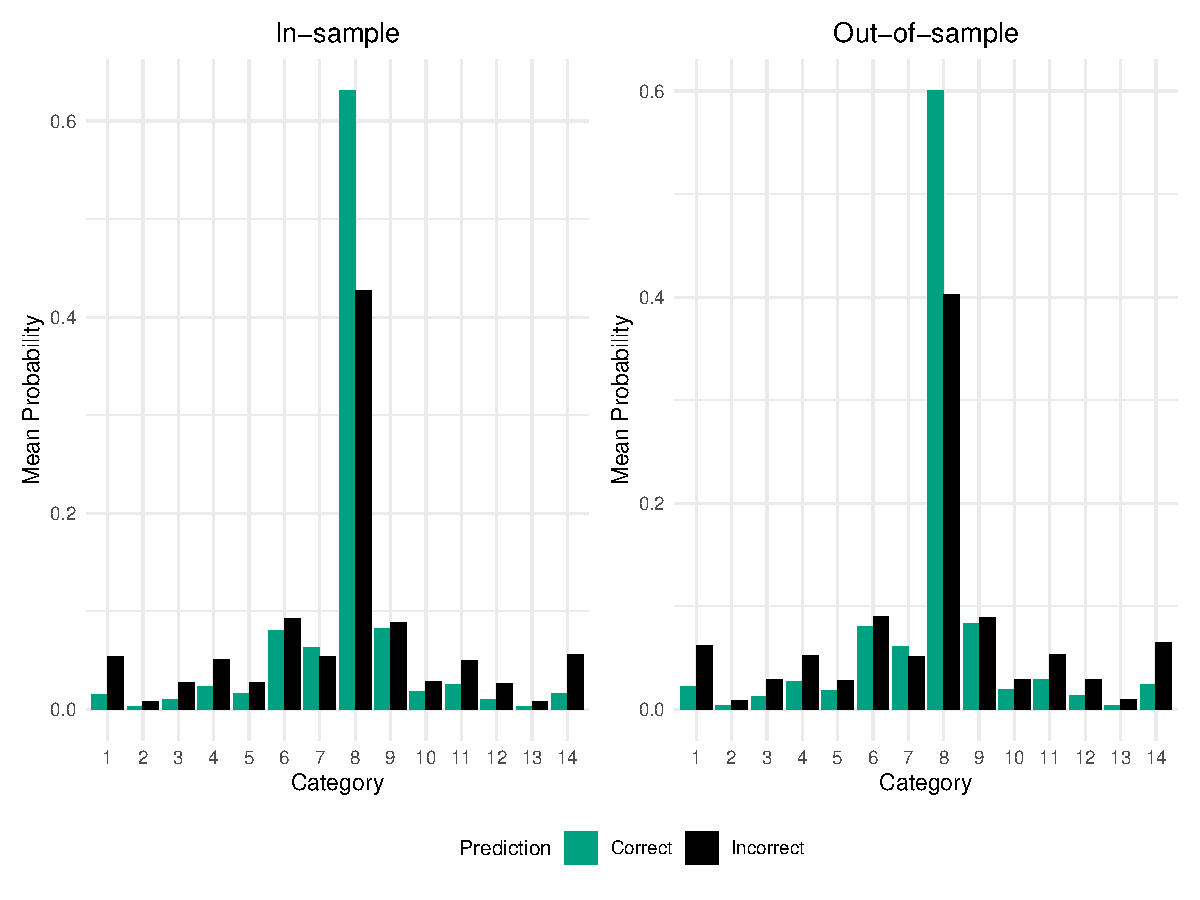
\includegraphics{figures/covid 19 period/overfitting_compare_covid.pdf}}
    \caption{Mean Probability by Prediction Class of In- and Out-of-sample (February-April 2020).}
    \label{fig:figure-6}
\end{figure}




\clearpage



\section{2008 Financial Crisis (September-October 2008)}

On September 15 2008, Lehman Brothers, back then one of the largest investment bank in the US, filed for bankruptcy. Following its collapse, the Dow Jones Industrial Average (DJIA) went down by 500 points on that trading day \citep{johnson&mamun2012}. This is one of the key events that have caused the global financial crisis lasting for roughly until 2008, or one could go with the "Great Recession" \citep{islam&verick2011}. For this thesis, the investigated period is from September 2 to October 31, with seven weeks for in-sample and two weeks for the out-of-sample forecast. A complete event study would need to look at a longer time period. Nevertheless, \tabref{tab:table-21} describes the sample size for this chosen period.

\tabref{tab:table-23} presents the distribution of price changes by tick as well as by our category's definition. Comparing to the previous case study of the recent Covid-19 pandemic, there are even more mass in the two tails. Moreover, further summary statistics of other $X_k$ variables are shown from \tabref{tab:table-22} to \tabref{tab:table-25} in Appendix \ref{app:tables-2008}. In overall, the trade direction proportion is roughly even between buyer-initiated (49.9\%) and seller-initiated (50.1\%). The bid/ask spread (mean of 0.08) is quite similar to the previous Covid-19 study (mean of 0.09), and both of these periods have wider spread than the main study's period (mean of 0.03).

Moreover, \tabref{tab:table-26} in Appendix \ref{app:tables-2008} reports the ordered probit model's estimation results. Accordingly, when roughly comparing with our previous studies in 2023 and Covid-19 2020, this model performs worst with McFadden's $R^2$ of only 0.0252. Only the first lag of price changes estimate is statistically significant at 0.1\% level as in the main study, while the second is only significant at 5\% level, and the third lag coefficient is not statistically significant.


\begin{table}[H]
\centering
\small
\renewcommand{\arraystretch}{1.3} % Increases row height
\setlength{\tabcolsep}{10pt} % Increases column separation
\resizebox{\textwidth}{!}{%
\begin{tabular}{|c|l|c|}
\hline
\textbf{Purpose}       & \multicolumn{1}{c|}{\textbf{Timeframe}} & \textbf{Number of transactions} \\ \hline
Panel E: Total         & September 2 - October 31, 2008          & 508,714                     \\ \hline
Panel F: In-sample     & September 2 - October 19, 2008            & 390,540 (77\% of total sample) \\ \hline
Panel F: Out-of-sample & October 20 - October 31, 2008          & 118,174 (23\% of total sample)   \\ \hline
\end{tabular}%
}
\caption{Summary of Database: IBM traded on NYSE (September-October 2008).}
\label{tab:table-21}
\end{table}



\begin{table}[H]
  \centering
  \setlength{\tabcolsep}{4pt} 
  \resizebox{\textwidth}{!}{%
    \begin{tabular}{@{} r *{14}{r} @{}}
      \toprule
      \textbf{Category}      & 1    & 2       & 3       & 4       & 5       & 6       & 7       & 8       & 9       & 10   
      & 11      & 12      & 13      & 14      \\
      
      \textbf{Price Changes}   & <–6  & [–6,–5) & [–5,–4) & [–4,–3) & [–3,–2) & [–2,–1) & [–1,0)  & [0,1)   & [1,2)   & [2,3)   & [3,4)   & [4,5)   & [5,6)   & \geq6     \\
    
      \textbf{Percentage} & 6.53\% & 0.79\% & 3.48\% & 4.95\% & 1.99\% & 9.98\% & 4.10\% & 40.81\% & 9.70\% & 1.98\% & 4.95\% & 3.50\% & 0.80\% & 6.44\%\\
      \bottomrule
    \end{tabular}%
  }
  \caption{Frequencies of Partition (September-October 2008).}
  \label{tab:table-23}
\end{table}



The test statistic for the effect of order flow is performed and presented in \tabref{tab:table-27} with statistical significant result that is able to reject the null hypothesis. In summary, throughout all of our three case studies, our model' results show consistent support for \citet{easleyohara1987} "information-effect" theory.





\begin{table}[H]
    \centering
    \vspace{0.5em}
    \begin{tabular}{crrl}
        \toprule
        Df & $\chi^2$ & Pr($>$$\chi^2$) \\
        \midrule
         2 & 135.71 & $<$ 2.2e-16 *** \\ 
         \bottomrule
        \multicolumn{3}{l}{$^{***}p < 0.001$; $^{**}p < 0.01$; $^{*}p < 0.05$}
    \end{tabular}
        \caption{Sequence of Trade: Linear Hypothesis Test (September-October 2008).}
    \label{tab:table-27}
\end{table}

Moving on to the impact of trade size on the next price change, \tabref{tab:table-28} presents the expected price impact for our dollar volume scenarios. Besides the similar trend of the larger volume the larger the impact, as noted for the Covid-19 period, the absolute impact in ticks for increasing amount of dollar volume for this "Great Recession" period is even greater. Again, conditioning for the increasing price sequence scenario and the base price of \$500, an increase of \$1000 trading volume in our financial crisis 2008 period would increase the conditional mean by 0.73 tick, while the impact of the previous studies are 0.33 tick (February-April 2020) and 0.19 tick (2023). A deeper analysis would needed to be able to investigate whether the seemingly decreasing in trade size impact due to the increasing liquidity of IBM stock through time, or it due to the effects of the crisis periods that cause the turbulence.







\begin{table}[H]
\centering
\begin{tabular}{lrr}
\toprule
 & \multicolumn{1}{c}{\$Volume} & \multicolumn{1}{r}{Impact} \\
\midrule
\multicolumn{3}{l}{\textbf{Increasing price sequence (1/1/1)}} \\
\addlinespace[0.5ex]
\multicolumn{3}{l}{\emph{Price impact in ticks}} \\
E$[Z_k]$             &  500   &  $-0.1707$ \\
$\Delta E[Z_k]$      & 1{,}000   &   $0.3654$ \\
$\Delta E[Z_k]$      & 1{,}500   &   $0.7286$ \\
$\Delta E[Z_k]$      & 2{,}000   &   $1.0898$ \\
$\Delta E[Z_k]$      & 2{,}500   &   $1.4490$ \\
$\Delta E[Z_k]$      & 5{,}500   &   $3.5094$ \\
\addlinespace[1ex]
\multicolumn{3}{l}{\emph{Price impact in percent}} \\
E$[Z_k]$             &  500   &  $-0.0017$ \\
$\Delta E[Z_k]$      & 1{,}000   &   $0.0036$ \\
$\Delta E[Z_k]$      & 1{,}500   &   $0.0072$ \\
$\Delta E[Z_k]$      & 2{,}000   &   $0.0107$ \\
$\Delta E[Z_k]$      & 2{,}500   &   $0.0143$ \\
$\Delta E[Z_k]$      & 5{,}500   &   $0.0346$ \\
\midrule
\multicolumn{3}{l}{\textbf{Constant price sequence (0/0/0)}} \\
\addlinespace[0.5ex]
\multicolumn{3}{l}{\emph{Price impact in ticks}} \\
E$[Z_k]$             &  500   &  $-0.1550$ \\
$\Delta E[Z_k]$      & 1{,}000   &   $0.3653$ \\
$\Delta E[Z_k]$      & 1{,}500   &   $0.7284$ \\
$\Delta E[Z_k]$      & 2{,}000   &   $1.0895$ \\
$\Delta E[Z_k]$      & 2{,}500   &   $1.4487$ \\
$\Delta E[Z_k]$      & 5{,}500   &   $3.5072$ \\
\addlinespace[1ex]
\multicolumn{3}{l}{\emph{Price impact in percent}} \\
E$[Z_k]$             &  500   &  $-0.0015$ \\
$\Delta E[Z_k]$      & 1{,}000   &   $0.0036$ \\
$\Delta E[Z_k]$      & 1{,}500   &   $0.0072$ \\
$\Delta E[Z_k]$      & 2{,}000   &   $0.0107$ \\
$\Delta E[Z_k]$      & 2{,}500   &   $0.0143$ \\
$\Delta E[Z_k]$      & 5{,}500   &   $0.0346$ \\
\bottomrule
\end{tabular}

\caption{Impact of Trade Size (September-October 2008).}
\label{tab:table-28}
\end{table}


\begin{table}[H]
\centering
\begin{tabular}{@{}lcc@{}}
\toprule
\multicolumn{1}{c}{Metric} & \multicolumn{1}{l}{\textbf{\% Accuracy}} & \multicolumn{1}{l}{\textbf{Hand-Till Multiclass AUC}} \\ \midrule
\textbf{In-sample}         & 41.47 \%                                 & 0.5661                                                \\
\textbf{Out-of-sample}     & 38.65 \%                                 & 0.5796                                                \\ \bottomrule
\end{tabular}
\caption{Forecasts Evaluation for In- and Out-of-sample (September-October 2008).}
\label{tab:table-29}
\end{table}

Last but not least, the forecasting performance of the our ordered probit model is also the worst among studies' periods, with both in-sample and out-of-sample \% accuracy below 50\% reporting in \tabref{tab:table-29}. The model undoubtedly needs further refinement to be robust for different time periods.






\begin{figure}[H]
    \centering
    \resizebox{0.85\textwidth}{!}{%
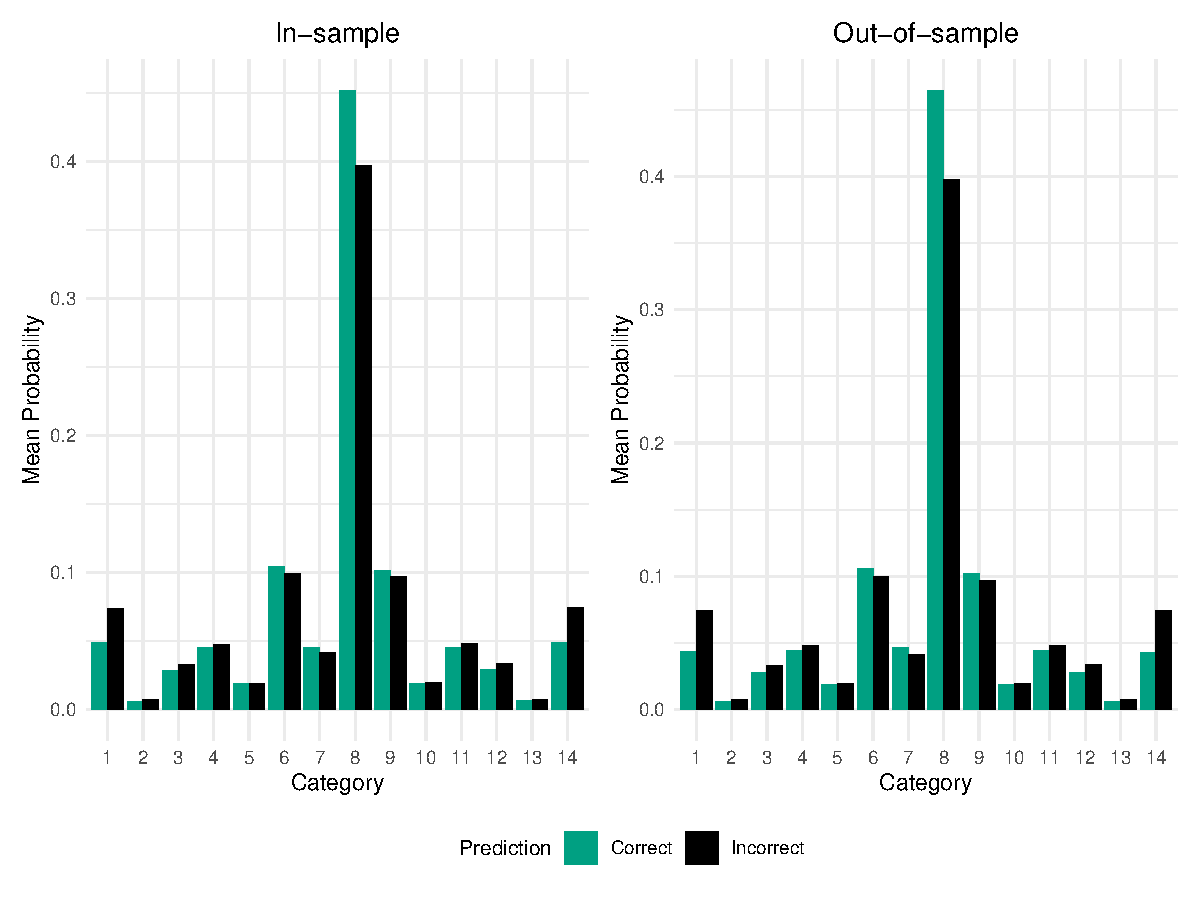
\includegraphics{figures/2008 financial crisis/overfitting_compare_2008.pdf}}
    \caption{Mean Probability by Prediction Class of In- and Out-of-sample (September-October 2008).}
    \label{fig:figure-7}
\end{figure}
